% \newpage

\section{Definição de Problemas Principais}

\subsection{Análise dos problemas}
O projeto tem por finalidades focar em alguns problemas do campus do Gama da Universidade de Brasília (FGA) a fim de que haja soluções compatíveis e viáveis. A proposta de aplicação do Smart Grid junto às fontes renováveis (solar e biogás), está sendo desenvolvida para combater esses impasse.
\par Os principais problemas encontrados foram  a dependência energética de apenas uma concessionária e o fato do consumo mensal de energia não ser compatível com o contrato feito com a empresa responsável pelo abastecimento energético no campus. Esses problemas serão discutidos a seguir.

\subsection {Consumo incompatível com o contratado} 
Tomando como base as contas de energia do campus no período de abril de 2015 à abril de 2016 e o consumo diário de energia elétrica, notou-se que os gastos com  eletricidade estão incompatíveis com os limites pré-estabelecidos no contrato entre a UnB e a CEB. Esse acorde determina uma quantidades de quilowatts(kW) a ser gasta mensalmente, o que por sua vez também determina um valor a ser pago de acordo com essa quantidade.
\par A partir desse valor fixado, definido como valor limite ponta, foi-se analisado que em determinadas épocas houveram alguns registros acima do valor limite ou com valor significativamente menor. Essa análise é ilustrada a seguir:
\begin{figure}[!htb]
\centering
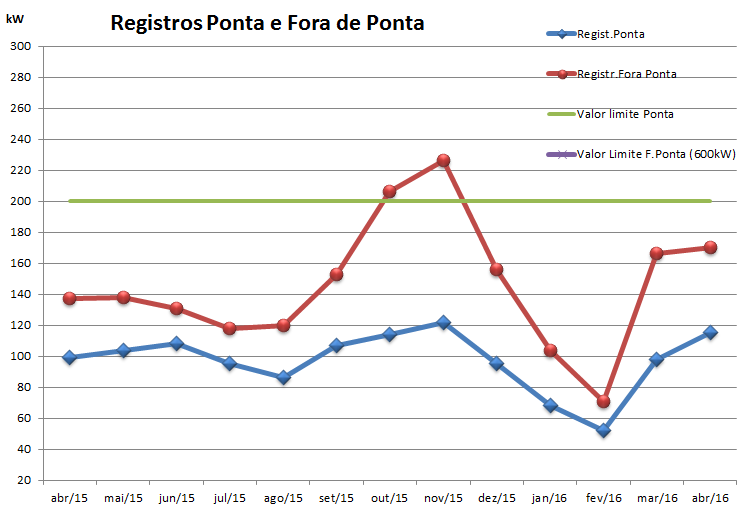
\includegraphics[width=0.6\paperwidth]{figuras/graficopontas.png}
\caption{Consumo (kW) x Tempo (meses)}
%\label{Rotulo}
\end{figure}

\par Percebendo que o consumo de ponta está sendo muito menor que o valor limite(600kW), valor fixado entre FGA e CEB, caso passe será cobrado um taxa de juros e multa e isso acaba gerando um desperdício para FGA, onde ela está pagando por um valor fixo muito alto que não será alcançada mesmo com seu mês de maior consumo, pois o maior consumo foi de 120KW, chegando a 20\% (vinte por cento) do valor fixado. A imagem \ref{fig:consumo} mostra o consumo de energia elétrica no período levantado:
\begin{figure}[!htb]
\centering
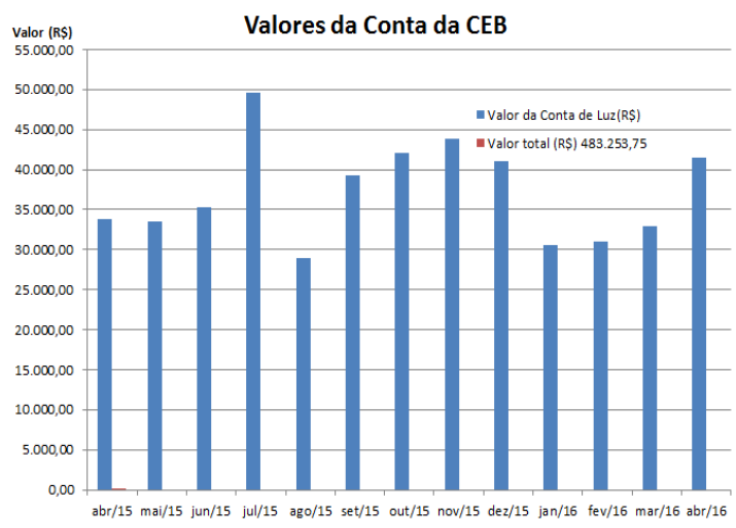
\includegraphics[width=0.65\paperwidth]{figuras/graficocontasCEB.png}
\caption{Consumo entre abril de 2015 e abril de 2016}
\label{fig:consumo}
\end{figure}



\subsection{Dependência da concessionária de energia elétrica}
Um dos grandes e mais evidentes problemas encontrados condiz da dependência da instituição com a concessionária de fornecimento da eletricidade.
\par O serviço de distribuição de energia elétrica é considerado, na literatura econômica, como um exemplo clássico de monopólio natural. Uma atividade econômica dá origem a uma estrutura de mercado de monopólio natural quando a produção é mais eficiente do ponto de vista técnico e econômico quando há apenas uma firma atuando no segmento específico do mercado \cite{ramos2012porque}
\par Sendo assim, por se ter uma única empresa disponível para o fornecimento da eletricidade e do serviço de manutenção desta, pode-se dizer que nas imediações da instituição existe um monopólio natural. Nesse caso, tem-se que a CEB - Companhia de Elétrica de Brasília - exerce um monopólio de serviço e fornecimento, não existindo uma concorrência sadia ou qualquer que seja. Isso acaba prejudicando diretamente a instituição pela necessidade de consumo e impossibilidade de comprar livremente de uma concessionária de sua escolha.
\par Não obstante, na ausência da ação do Regulador, o monopólio natural em nada beneficia os consumidores. Se há apenas uma firma atuando no setor e se encontra naturalmente protegida da competição, a tendência é que prevaleçam altos preços de serviços que se traduzirão em lucros extraordinariamente elevados para o monopolista. Esta possibilidade concreta justifica que atividades que são reconhecidas como monopólios naturais sejam usualmente reguladas com o objetivo de proteger o consumidor contra a prática de preços elevados \cite{ramos2012porque}.